%% Standard article template by Geir Isene (2012-04-05)

%% Document basics
\documentclass[11pt]{article}
\usepackage[margin=2cm]{geometry}

%% Fancy headers
\usepackage{fancyhdr}
\pagestyle{fancy}
\fancyhead[LE,RO]{\thepage}
\fancyhead[RE]{\thetitle}
\fancyfoot{}

%% Endnotes
\usepackage{endnotes}
%\let\footnote=\endnote

%% Language, hyphenation
\usepackage[english]{babel}
%% No-hyphenation: Usage = \nohyphens{text...}
\usepackage{hyphenat}

%% Graphics and colors
\usepackage{graphicx}
\usepackage[usenames]{color}
\definecolor{r}{rgb}{0.5,0,0}
\definecolor{g}{rgb}{0,0.5,0}
\definecolor{g2}{rgb}{0,0.2,0}
\definecolor{b}{rgb}{0,0,0.5}
\definecolor{v}{rgb}{0.4,0,0.4}
\definecolor{t}{rgb}{0,0.4,0.4}

%% Numbering "paragraps" (as subsubsubsection)
\setcounter{secnumdepth}{5}
\setcounter{tocdepth}{5}
\makeatletter
\renewcommand\paragraph{%
  \@startsection{paragraph}{4}{0mm}%
   {-\baselineskip}%
   {.5\baselineskip}%
   {\normalfont\normalsize\bfseries}}
\makeatother

%% Creating deep lists
\usepackage{enumitem}
\setlistdepth{9}
\setlist{noitemsep}
\newlist{deeplist}{itemize}{9}
\setlist[deeplist]{label=\textbullet}

%% Math environment
\usepackage{amsmath}
\renewcommand{\theequation}{\roman{equation}}

%% Various packages
%% Nicer scalable fonts
\usepackage{pslatex}

%% Verbatim that recognizes LaTeX commands
\usepackage{alltt}
\renewcommand{\ttdefault}{txtt}

%% Hyperlinks
\usepackage[breaklinks=true,bookmarks=true,bookmarksopen=true,pdfpagemode=None,pdfstartview=FitH,colorlinks=true,citecolor=v,urlcolor=v]{hyperref}

%% Nicely format and linebreak URLs in the bibliography (and elsewhere).
\usepackage{url}

%% Allow relative font size specifications (e.g. \smaller, \larger).
\usepackage{relsize}

%% Shortcut commands
\newcommand{\hyperlist}{H{\sc yper}L{\sc ist}\textsuperscript{\tiny{S}}\hspace*{0.2em}}
\newcommand{\tb}{\hspace*{0.1em}}
\newcommand{\bi}{\begin{itemize}\itemsep1pt}
\newcommand{\ei}{\end{itemize}}
\newcommand{\be}{\begin{enumerate}\itemsep1pt}
\newcommand{\ee}{\end{enumerate}}
\newcommand{\bdl}{\begin{deeplist}}
\newcommand{\edl}{\end{deeplist}}
\newcommand{\bv}{\vspace{-4mm}\begin{alltt}\begin{textbf}}
\newcommand{\ev}{\end{textbf}\end{alltt}}

%% Front page
\title{On Will\\{\small Do you have a choice?}}
\author{Geir Isene\\{\small g@isene.com}\\{\small \url{http://isene.com}}\\\\{\small \em{editing}}\\{\small Marilyn Abrahamian}} 
\vspace{20mm}
\date{{\small Version: 2.5 (2016-02-09)}}


%% START OF ARTICLE
\begin{document}

\maketitle
\begin{center} 
License: CC by-sa
\end{center}

\vspace{20mm}

\begin{center} 
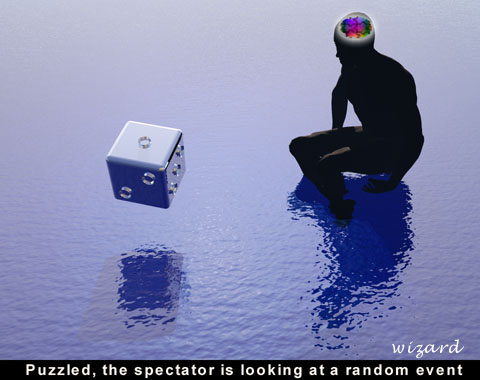
\includegraphics[trim = 0mm 15mm 0mm 0mm, clip, width=100mm]{random}\\
{\bf {\em Puzzled, the spectator is looking at a random event.}}
\end{center}

\vspace{40mm}

\begin{center}
{\small Document link: \url{http://isene.me/free-will/}}
\end{center}

\newpage
\begingroup
\hypersetup{linkcolor=v}
\tableofcontents
\endgroup

\vspace{15mm}

\begin{abstract}
This article attempts to shed light on existential questions like {\em ``Does
free will exist?'', ``Do you have a choice?'', and ``If you can exercise will,
how can that affect the reality we perceive?''} The article also looks at the
possible relation between free will and quantum mechanics.
\end{abstract}

\newpage
\section{Do you really have a choice?}

On the subject of choice, there are two options: Either you really have a
choice, or the appearance that you may choose is simply an illusion.

By {\em choice} is meant the possibility of {\em will} being exercised.
Thus, the subject of choice is strongly related to the subject of free will. Do
you really possess free will?

Since there are many situations where people seemingly cannot choose what they
want, we will refer to free will as meaning potential free will.

You either have potential free will or no free will. In the latter case, it
should not even be called {\em will} as everything is then simply a series of events
with no will involved.

Let us explore the possibility of no free will: You have no choices; it is all
out of your control. Everything is simply a series of events. There is no will
involved and everything is determined by the laws of the physical universe. This
assertion we label a {\em Physical Theory} or an {\em Objective Theory}.

Determinism is a common view among natural scientists and is gaining ground in the
general population. In the book {\em A Brief History of Time}\footnote{{ \em A
Brief History of Time}:
\url{http://en.wikipedia.org/wiki/A\_Brief\_History\_of\_Time}}, the
astrophysicist Steven Hawking explains it very well: If you know the state of
the universe at any given time and all the laws that govern it, you can
calculate all consecutive events. You can determine every single motion in the
universe at any time. The brilliant French scientist Pierre-Simon Laplace
formulated this idea in a paper published in 1814\footnote{{ \em A Philosophical
Essay on Probabilities} (eng. 1902):
\url{http://www.archive.org/details/philosophicaless00lapliala }}. Although it
has been proven that such a thought experiment is impossible\footnote{ P.-M.
Binder, ``Theories of almost everything'', Nature, 455 (2008), 884-885}, that
proof still does not disprove the universe as causally deterministic.

Many physicists disagree with Laplace in that they assert the possibility of
randomness in the universe. Random events would break the prospect of
calculating the future. However, randomness does not itself leave room for any
will or real choices.

We see that there are two Objective Theories: the Deterministic Model and
the model that allows for random events, the Random Model.

The Objective Theories are attractive in that they present complete systems
within the boundaries of the physical universe without any external influence.
The beauty of such a system lies in what it can prove -- anything physical can
be proven in and by the physical universe.

The Objective Theories also make the science of physics the ultimate profound
science able to explain it all.

However, Ludwig Wittgenstein\footnote{ Ludwig Wittgenstein: 
\url{https://en.wikipedia.org/wiki/Wittgenstein }}
noted, as a corollary to G\"{o}del's Incompleteness Theorems\footnote{ G\"{o}del¿s Incompleteness Theorems:
\url{http://en.wikipedia.org/wiki/G\%C3\%B6del\%27s\_incompleteness\_theorems
}}, that all the facts of science are not enough to understand the world's
meaning, because ``The meaning of the world does not reside in the
world''\footnote{ ``Logicomix'' by Apostolos Doxiadis and Christos Papadimitriou:
\url{https://en.wikipedia.org/wiki/Logicomix }}.

In the Objective Theories, there is no {\em will} that can cause anything.
Everything is an effect of an earlier effect or is simply a random event. With
no will there is never any purpose behind why something happens.

If the world view of {\em no free will} is the truth, it has ramifications into most
fields of human endeavor. It most obviously disrupts the field of religion as
religions in the main build on the notion of free will and the possibility of
choices. But it also disturbs the fields of philosophy, ethics and law. With
the removal of the concept of will comes the subtraction of responsibility.

\newpage

Aristotle outlined the essence of responsibility -- a definition that remains
the basis for accountability in our judicial systems\footnote{ ``Moral
Responsibility'' by Andrew Eshleman:
http://plato.stanford.edu/entries/moral-responsibility/}:

\begin{quotation}
   \em ``Aristotle's discussion is devoted to spelling out the conditions under
   which it is appropriate to hold a moral agent blameworthy or praiseworthy for
   some particular action or trait. His general proposal is that one is an apt
   candidate for praise or blame if and only if the action and/or disposition is
   voluntary. According to Aristotle, a voluntary action or trait has two
   distinctive features. First, there is a control condition: the action or
   trait must have its origin in the agent. That is, it must be up to the agent
   whether to perform that action or possess the trait -- it cannot be compelled
   externally. Second, Aristotle proposes an epistemic condition: the agent must
   be aware of what it is she is doing or bringing about.''
\end{quotation}

There is no accountability for actions if there is no will behind them. There is
no one to be held responsible if the person had no choice. Thus, the human
systems of law and order are merely illusions -- as is the apparent drive for
happiness or attaining one's goals. All such pursuits are appearances that are
bound to happen or happen by chance. The appearance of choice is an illusion.
There is no reason for living.

The nullification of responsibility may seem glum to some and a relief
to others. But it hardly matters as it either seems that way due to
chance, or it was bound to happen.

There is no wrongness or rightness in the Objective Theories. There is only
{\em isness}.

In the Objective Theories, there is no real difference between a human, an animal
and a well-crafted robot. Artificial intelligence is within reach.

The physical universe is composed of space, energy, matter and time. Everything
within it is governed by its laws, whether the laws allow for random events or
not. Therefore, in order for free will to exist, it cannot be governed by the
laws of the physical universe, just like Wittgenstein noted.

The power of choice must at least in part be separate from the physical universe
in some way. And only if it can potentially be completely separate can it
potentially be fully free. Free implies free from space, energy, matter and
time. It does not suggest that free will is somehow {\em physically} located
outside the universe as that would still subject the will to physical laws and
hence it would not be free.

Let's explore a theory of free will: You can choose. It is up to you. You can
change the course of events. You are accountable for your actions and are
ultimately responsible. This assertion can be labeled a {\em Metaphysical
Theory} or a {\em Subjective Theory}.

Again, this may seem glum to some and a relief to others.

Free will imposes changes on the physical universe if only on a very small
level, perhaps much like the {\em butterfly effect}\footnote{ The butterfly
effect: \url{http://en.wikipedia.org/wiki/Butterfly\_effect}}.

Free will introduces the {\em observer} into the universe, an element that seems
to fit well with quantum mechanics. Lee Smolin, in the book {\em The Trouble
with Physics,} lists the five great problems facing the science of physics
today. The second problem reads: ``{\em Resolve the problems in the foundation
of quantum mechanics, either by making sense of the theory as it stands or by
inventing a new theory that does make sense}\footnote{ Lee Smolin, 2006, {\em The
Trouble with Physics}, Houghton Mifflin Harcourt, p. 8}''. The external observer
possessed with free will could resolve the problems in the foundation of quantum
mechanics, as will be explored later in the article.

As free will lies outside the realm and laws of the physical universe and acts
as an external influence, it cannot be directly proven or disproved in and by
the physical universe. Any proof can only be circumstantial. For that reason,
the weakness of this theory is that it cannot be proven to those who will accept
only direct physical proof of a phenomena.

As free will is exterior to the laws of the physical universe, it supersedes
time. Hence, it was never created and will never be destroyed. It may or may not
be the cause of the physical universe but it was not caused by it. In fact, free
will cannot be caused by the physical universe as nothing can beget something
outside its realm of influence. Or in a simpler form: {\em Nothing can beget
something with greater potential than its own}. This would rule out the
possibility of creating real artificial intelligence. AI may certainly mimic
free will and thus create the illusion of a computer possessing free will;
however, it cannot transcend the laws of the universe in which it exists.

A definition of pure potential free will could be ``cause without prior cause''
or the equivalent, ``cause without reason''.

Even though free will is exterior to the physical universe, it is influenced by
it to a varying degree. It loses its potential in ratio to its identification
with the physical universe. This may explain the varying degree of apparent free
will.

If a Subjective Theory is true, it poses the question of whether a belief in
an Objective Theory would be a self-fulfilling prophecy. On the other hand, if
an Objective Theory is true, a belief in a Subjective Theory would merely be
a belief in an illusion for which the person bears no responsibility. Another
question that can be posed is, who would be relieved by which theory? I will
leave this for the reader to ponder.

According to Wikipedia\footnote{ Cognitive dissonance: \url{https://en.wikipedia.org/wiki/Cognitive_dissonance}}: 
``In psychology, cognitive dissonance is the mental stress
or discomfort experienced by an individual who holds two or more contradictory
beliefs, ideas, or values at the same time, performs an action that is
contradictory to one or more beliefs, ideas or values, or is confronted by new
information that conflicts with existing beliefs, ideas, or values.''

To avoid cognitive dissonance, one would be well advised to act according to
one's beliefs. Thus, if one believe in free will, then one should act
accordingly, accepting responsibility for one's actions. If one does not believe
in free will, then there is no responsibility or accountability or purpose in
life and one should act accordingly. If one would want to avoid the cognitive
dissonance.

It is worth noting that in this discussion of free will, one could simply reduce
it to a discussion of whether {\em will} exists at all. If the answer is {\em
yes}, reality cannot be purely deterministic and/or random. {\em Will} is that
other factor beyond determinism and quantum randomness.

Whether you choose to believe in an Objective or Subjective Theory may not
really be a question at all. If an Objective Theory is true, your belief is not
your choice to make. If a Subjective Theory is true, it is either you choosing
to see the truth or your choice to disregard the truth and thereby possibly
make yourself even more subject to physical laws.

The choice may or may not be yours.

\newpage

\section{Can the universe be deterministic?}

As noted earlier, determinists believe the universe is fully governed by causal
laws resulting in only one possible state at any point in time. But can the
universe actually be causally deterministic? Let's see:

\begin{enumerate}
	\item For a system to be deterministic, its underlying rules must be consistent.
	\item For a system to be deterministic, its underlying rules must be complete.
	\item No system of rules can be both complete and consistent per G\"{o}del's Incompleteness Theorems	
   \item Thus, no system can be deterministic.
\end{enumerate}

This would rule out Laplace's idea of the universe being causally deterministic.
What is left, then, of the Objective Theories is the Random Model, allowing for
either the incompleteness or the inconsistency made inevitable by G\"{o}del's
Incompleteness Theorems.

In addition to being the basis of proof that no system can be deterministic,
G\"{o}del's Incompleteness Theorems show that it is impossible to prove the
Physical Theory in and of itself.

No consistent universe is ever complete. There would always be another factor or
axiom that would explain it further. Thus, the physical universe cannot be
everything there is if it is to remain consistent. There must be some other
factor beyond it that gives it meaning.

The full and complete reassurance, the comforting certainty about why things
happen, seems more elusive than ever. But the absolution from all responsibility
may still be feasible through the Random Model.

In the section ``Cause and Effect'', we will explore what a Subjective Theory
could entail.

\section{Extrapolating Free Will}

If there exists potential free will, free of any physical restrictions, that
free will cannot have been created as time is a physical property. Thus, free
will supersedes the physical universe, or has always co-existed with the
physical universe if the universe has no beginning. The latter could be
challenged by such questions as ``Can anything physical exist that wasn't
created?'' and ``Can any effect exist that wasn't caused?''

As free will causes changes in the physical universe, it represents the {\em
cause}; and space, energy and time are the {\em effect} of free will acting.

The physical universe is truly {\em effect} and is not capable of causing
anything -- it has no will of its own. Free will, on the other hand, cannot be
affected by anything except by its own choice, as it is by its nature
potentially free from the laws of the physical universe. That potential is
alloyed solely by the individual's own considerations. Therefore, anything that
free will experiences is by its own volition. By choosing otherwise, free will
experiences otherwise.

While the physical universe is total effect, free will is cause. Although free
will makes choices by its own volition, its choice may be swayed by its
experiences, which are the result of its choices. 

A feedback mechanism is then seen as free will chooses its own experiences and
is then affected by them. This may lead to free will apparently losing control
of its will by association with the physical universe and believing it has less
free will. It will then act less free, less {\em cause}. To change this feedback
mechanism, free will can be persuaded, perhaps by another free will, to believe
it is more {\em cause} and less {\em effect} and thereby bring the situation under
the power of will once again.

Any persuasion masked as a solution may -- do as long as free will believes the
solution presented will work and as long as the solution aligns with physical
universe laws to the degree that the individual believes in those laws. This may
explain how many people are helped by a wide plethora of practices aimed at
bettering the individual. It may also explain the placebo effect.

\section{Cause and Effect}

A realist believes in the RWOT (the Real World Out There)\footnote{ Lee Smolin,
2006, {\em The Trouble with Physics}, Houghton Mifflin Harcourt, p. 7 }, the
universe existing wholly independent of its harboring observers. This branch of
thinking is called ``philosophical realism''.

An alternative view is that of the RWIH (the Real World In Here)\footnote{ RWIH
(Real World In Here): Coined by the author}, the universe being a consensus
reality of the wills involved in creating it.

Suppose potential free will is capable of creating a complete reality on its own
-- like what most people experience when they are dreaming. While there is
enjoyment in playing a variety of solitaire-type games, there can be more
enjoyment in playing games where other wills are involved as this creates a
balance of cause and effect for oneself. Hence the creation of a consensus reality.

The physical universe may be seen as a common ``playing ground'', where each
participant contributes his own visions and realities but where everyone agrees
on a set of rules, including the laws of physics.

If a potential free will is only affected by its own considerations, how can it
then know about other potential free wills? One explanation could be that there
exists a Potential for cause and free wills emerge from this Potential Cause.
With a common source, separate free wills could inherently be linked.

Think of the Potential Cause as a blank piece of paper. From this paper arise
points (separate cause points) that decide to BE (able to draw on the paper).
Each point draws its own small picture (its own universe). As two points
interact with their drawings, they start creating a common reality. As
additional points interact with their drawings, a broader consensus reality
emerges.  Wikipedia is an example of such a co-created reality, as is the
virtual world of Second Life\footnote{ Second Life: \url{https://en.wikipedia.org/wiki/Second_life}}

Individuals emerging from a Potential Cause parallels what is seen in particle
physics, where the potential of space gives rise to pairs of
particle-antiparticle.

The Cause is pure potential. From this Cause then come decisions {\em to BE},
with each individual having its own reality or universe through its own
considerations. Each such individual basically {\em is} his own universe with
all its considerations. Individuals have the power of limitless consideration.

Each individual has the potential to cause effects through considerations.
Nothing exists beyond what is considered. Anything existing is due to
considerations.

A consideration is a decision. And every consideration creates an effect, as it
is motivated by the ability to cause. Each represents a desire for something
and, to a certain degree, puts that desire into effect, giving rise to new
considerations that move one closer to the desired something. 

For every consideration, there is cause creating effect, making for the fractal
structure of universes. As considerations are added, layer upon layer, the very
basic considerations, the ``trunk'' of the ``tree of considerations'', grows more
elusive as ``branches'' and ``leaves'' cover the view of it.

To create the consensus reality we know as the physical universe, it requires a
massive quantity of considerations -- all the way from the basic laws of physics
up through the way these laws allow for combinations of basic forms into
structures, and further up to how each individual interacts with the physical
universe through a body -- and even further up to creating a life within the
consensus reality. With an enormous number of individuals participating, each
with a vast quantity of considerations, the complexity of the physical universe
can be rather staggering.

To be part of a common {\em playing ground}, individuals must obey the rules of
the consensus reality.

It is much like any other game, like soccer, for example -- to participate one
must abide by the rules. As the individual participates in the consensus reality
(the physical universe), he takes on a massive amount of agreement with those
rules. An individual is bound by the agreements of the physical universe.
Hence, he ordinarily cannot simply lift an object by pure consideration unless
he solicits agreement by all individuals in the consensus reality -- or unless
it is somehow allowed by the rules. This may explain the lack of commonly
displayed psychic abilities. It may also explain magic (i.e. someone found a
buried allowance for certain magic to be displayed, or a loophole in the rules).

If such a Subjective Theory is true, then one would expect to see, from time to
time, a variety of phenomena such as OBE (out-of-body experience) and remote
viewing. Most realists would have abandoned this article well before this
paragraph, perhaps by preconceptions or emotional stands. A Subjective Theory
would, however, offer explanations for phenomena that an Objective Theory cannot
satisfactorily explain or which it unscientifically dismisses altogether. But to
be complete, a Subjective Theory will have to offer further testable predictions
as well as possibilities for falsification.

An individual existing within the consensus reality is very much at apparent
effect simply because of his agreement to the rules. He may apparently become
even more effect by agreeing further to others' considerations -- by taking them
on as his own. Layers upon layers of considerations result in lower levels being
masked by higher levels. The lower-level considerations can then be referred to
as {\em unconscious considerations}.

There is a gradient scale of free will that shows how much an individual is in
agreement. For an individual to rise on this scale, a solution must be presented
matching the individual's level of agreement. A heavy drug addict, heavily into
agreement with physical universe laws and others' considerations (basically the
same thing), needs a very physical solution in order for him to accept its
workability.  An individual high on the scale needs the simplest of solutions
-- like what is described by the British philosopher Alan Watts when he
relates why any practice of individual improvement can work. He says that the
only reason an Eastern guru would ask someone to go through a regimen of mental
and physical exercises is that they cannot simply ``{\em get off it}'' -- they
need to feel they deserve the insights before they attain them\footnote{ Alan
Watts' video: \url{http://www.youtube.com/watch?v=fCSsiF3BQoQ}}.

As an individual is only bound by his own considerations and can only be hurt or
become effect by his own considerations, resolving his own considerations is
essentially the only solution there is. This may, then, explain why placebos
work -- an effect medical societies should embrace wholeheartedly. Any solution
works only to the degree that it can entice the individual into considering that
it will work.  This is why any religion can work, as can psychotherapy, or
psychiatry, faith healing, meditation, or simply anything, as long as the
individual considers it will work. With this understanding comes tolerance of
others' realities, of other religions and views. 

Some techniques reach the level of agreement of more people than other
techniques. Workability is further enhanced by the individual's perception of
the value of the solution. If the solution includes much suffering, monetary
cost, secrecy or scarcity, it will often be seen as more valuable and hence has a
better potential of getting some individuals to accept it as workable.

As any solution can work and will work best if it strikes at the level of free
will exercised by the individual, there is a scale of solutions from the most
physical to the very light. Starting at the most physical levels, we have
solutions such as band aids, surgery, medicine, vitamins and on up through
various therapies and rituals to tackling the effects of the individual's most
intimate considerations. But above all of this would be addressing the
individual's considerations directly.

Instead of addressing the individual's perceived problem, one could address his
considerations about it, to release his free will. His considerations are, after
all, the only things anchoring him to the problem. Having him simply look at his
own considerations layer after layer should bring him to whatever level he
would like. 

There is evidence in physics supporting such a Subjective Theory as the one
outlined above. QM (quantum mechanics) hints at the observer being an active
ingredient in creating the reality we see.

\newpage
\section{A Subjective Collapse Theory}

What makes the quantum mechanics (QM) wave function collapse?

This has been one of the great questions giving work to physicists ever since
Erwin Schr\"{o}dinger came up with his mathematical explanation for
wave-particle duality. In the aftermath of the mathematics came philosophical
questions: Is the universe objective? Does it exist if we are not observing
it? Are there many universes? Coexisting?

Particles are waves and waves are particles. Simultaneously. Apparently they
are both until they are measured. Then they settle to become a particle. 
The famous double-slit experiment\footnote{ Double-slit experiment:
\url{http://physics.about.com/od/lightoptics/a/doubleslit.htm}} shows what is
known as a {\em wave function collapse}: the wave function describing the
probability of the particle's location collapses from probability to actuality.
The experiment suggests that the collapse is related to measurement by a
conscious observer.

This concept was taken further by the late John Wheeler in his {\em
delayed-choice} thought experiment. It postulated that measurements here and now
can influence and causatively determine the path that a photon has been
travelling for billions of years\footnote{ John Wheeler's delayed-choice thought
experiment: \url{http://discovermagazine.com/2002/jun/featuniverse}}. Such
perplexing ideas go back to Erwin Shr\"{o}dinger's thought experiment devised to
show the absurdity of some interpretations of QM. But when Schr\"{o}dinger put
forth his {\em Schr\"{o}dinger's cat} as an attempt at a reductio ad absurdum,
he only sparked a flurry of interesting interpretations.

Schr\"{o}dinger's cat describes a closed quantum system -- a box with a cat
inside.  The cat's life depends on whether a vial of poison gas is broken by a
hammer linked to a Geiger counter that may be triggered by a possible
radioactive emission from a small piece of uranium. The possibility of the
uranium having emitting a particle is what makes the system undecided until
someone opens the sealed box, observes and thereby collapses the quantum system.
The eminent physicist Eugene Paul Wigner extended the conundrum by asking when
the system is decided from the next person's perspective: when his friend (the
person in the laboratory) opens the box or when he is told whether his friend
found a dead cat inside. This extension is known as {\em Wigner's friend}. It
probes the philosophical boundaries to Schr\"{o}dinger's cat.

The interpretations of QM range from the strict deterministic, like some
Objective Collapse Theories claiming that all seemingly random events were
decided at the Big Bang, to theories accepting an inherent, unpredictable
randomness in the Universe, to the theory known as Consciousness Causes
Collapse. The latter is a version of Wheeler's Participatory Anthropic
Principle\footnote{ Wheeler's Participatory Anthropic Principle:
\url{http://www.abc.net.au/rn/scienceshow/stories/2006/1572643.htm}} and claims
that an observer is the active agent deciding the state of a quantum system by
observing and collapsing it. 

Further, in 2007, Wheeler's delayed-choice thought experiment was confirmed.  An
implementation of it suggests that the act of observation ultimately determines
whether the photon will behave as a particle or wave\footnote{ Delayed-choice
experiment:
\url{http://en.wikipedia.org/wiki/Wheeler's\_delayed\_choice\_experiment}}.

This moves the conundrum to the philosophical debate about the nature of consciousness.

Most criticisms of the idea of Consciousness Causes Collapse go along these lines:

\begin{quotation}
\em ``Was the wave function waiting to jump for thousands of millions of years
until a single-celled living creature appeared? Or did it have to wait a
little longer for some highly qualified measurer -- with a PhD?\footnote{ Bell, 
J.S., 1981, ``Quantum Mechanics for Cosmologists''. In C.J. Isham, R. Penrose and
D.W. Sciama (eds.), {\em Quantum Gravity 2: A Second Oxford Symposium}. Oxford:
Clarendon Press, p.611.}''
\end{quotation}

Such criticism suffers from a logical fallacy in that it carries a hidden
assumption: that consciousness must be physical, evolved in and contained within
the domain known as the physical universe. While it may seem obvious to some
that consciousness can only be in the domain of physics, it is nevertheless a
hidden assumption.

\newpage

Steven Weinberg wrote an article published in {\em Physics Today, November 2005,
titled ``Einstein's Mistakes''}\footnote{ ``Einstein's Mistakes'':
\url{http://scitation.aip.org/journals/doc/PHTOAD-ft/vol\_58/iss\_11/31\_1.shtml?bypassSSO=1}
}. He makes what seems like a good argument for why QM can indeed be treated
deterministically:

\begin{quotation}
\em ``The Copenhagen interpretation describes what happens when an observer
makes a measurement, but the observer and the act of measurement are themselves
treated classically. This is surely wrong: Physicists and their apparatus must
be governed by the same quantum mechanical rules that govern everything else in
the universe. But these rules are expressed in terms of a wavefunction (or,
more precisely, a state vector) that evolves in a perfectly deterministic
way.''
\end{quotation}

Unfortunately, Weinberg's argument suffers from the same logical fallacy as
noted above. His hidden assumption is quite visible when it starts with
{\em``This is surely wrong\ldots''} Weinberg's argument is only true if the
observer is in fact wholly within the domain of the laws governing quantum
mechanics.

If consciousness exists independent of the physical universe (or indeed any
physical universe), it may be the missing element in the reason for the wave
function collapse. This now introduces the {\em subject} (that which thinks,
feels, perceives, intends) in a Subjective Collapse Theory. This is the
observer, the individual mentioned earlier.

Before one dismisses the Subjective Collapse Theory on emotional grounds, it
should be noted that no theory is complete without having explored all possible
weaknesses and hidden assumptions. The possibility of an external subject
causing collapse should warrant investigation.

If free will exists, it must exist outside the physical domain and as such is
indeed an external observer of the quantum system known as the physical
universe. Even so, if a subject observing an event exists separate from the
physical universe, this does not necessarily imply that it possesses free will.
However, the case for free will has been argued earlier in this article.

Let's outline a Subjective Collapse Theory as a very simple \hyperlist
\footnote{ \hyperlist \url{http://isene.me/hyperlist/ }}. Note: the line in
green describes the conditions under consideration, and the word ``OR'' indicates
that indented below it are the possible situations.

\bv
   \textcolor{g}{["Schr\"{o}dinger's Cat" = True & "Subject needed for collapse" = True]}
      \textcolor{b}{OR:} 
         Quantum system undecided \textcolor{t}{(for you)}
            Particle possibly emitted 
            Particle possibly interacting with solid matter 
            System observed by cat 
         Quantum system decided \textcolor{t}{(for you)}
            Event observed by you as the subject 
      Each subject has its own reality 
      A common reality is created by interacting subjects
\ev

As you can see, this logical breakdown treats the Schr\"{o}dinger Cat's thought
experiment as true and not merely a reductio ad absurdum. Granting that the
experiment is true and the outcome is determined by a subject observing the
event, it follows that every subject has its own reality and what is
viewed as {\em objective reality} is then caused by subjects interacting.

Perhaps the quantum randomness we observe is really the result of subjects
possessing free will creating a consensus reality through their considerations.
With an enormous number of "players" in the game, and with every particle up for
debate, whether a certain particle goes left or right may seem completely
random, while in fact it could be the result of consensus considerations
tugging the physical ``reality''.

This is not an attempt at logically proving this Subjective Collapse Theory but
merely to propose it as a possible interpretation of quantum mechanics
\footnote{ Interpretations of QM: \url{http://en.wikipedia.org/wiki/Interpretation\_of\_quantum\_mechanics
}}. 

\newpage
\section{A final note: Unification}

The search for unification in physics has been a holy grail for centuries. A
Subjective Theory, including the Subjective Collapse Theory, would introduce a
unification of an order higher than that of physics. It would unify the natural
and social sciences; it would unify physics, psychology and philosophy and
their siblings.

It would also bring the notion of responsibility into every social science.

The question of unification in physics may boil down to the simplest of ideas:
that reality is reality by consideration only and that the laws of physics do
not constitute the most senior concept describing our universe. The
consideration that those laws exist would be the most senior concept. Beyond
that, there would be only Potential Cause, and this Potential Cause causes
effects simply because it can, and not as the effect of some other cause. In
that, one may speculate about
multiverses\footnote{ Multiverses: \url{http://www.daviddarling.info/encyclopedia/M/multiverse.html}}
as a possible logical result of pure Potential Cause.

This article does in no way comprise a complete theory. It simply outlines some
ideas for a theory, perhaps enough to spark some interest in looking at reality
as consensus considerations.

\vspace{10mm}
\begin{center}
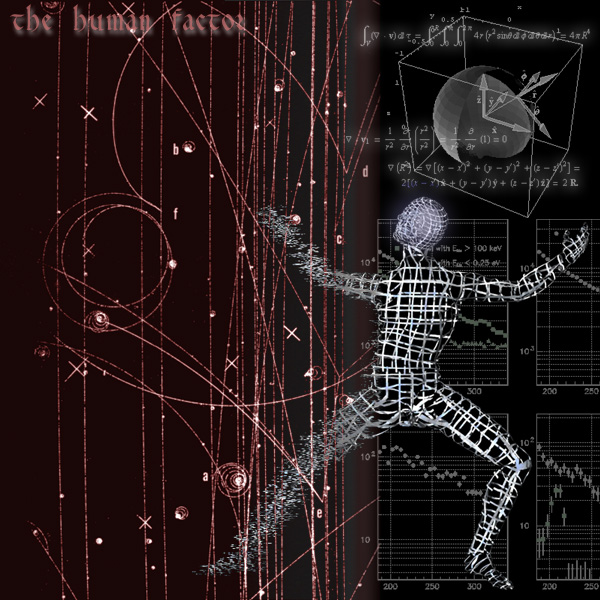
\includegraphics[width=50mm]{humanfactor}
\par\end{center}

\newpage
\begingroup
\parindent 0pt
\parskip 1ex
\def\enotesize{\small}
\theendnotes
\endgroup

\end{document}
